\chapter{Descripción de los modelos teóricos utilizados}
\label{descripcionmodelos}

\section{Modelo de rendimiento térmico de 4º Orden para caracterización de un sistema de captación solar}
El modelo de partida desarrollado en \cite{barberofresnoDesarrolloModeloTeorico2018} tiene un caracter general que permite que sea aplicado a receptores térmicos de radiación solar de cualquier tecnología, tanto para concentradores cilindroparabólicos como para conentradores lineales Fresnel o receptores de torre central. En este trabajo nos centramos en los aspectos relativos a los CCP y a continuación revisaremos las características del modelo para este tipo concreto de receptores.

El receptor considerado inicialmente consiste en un tubo desnudo de diámetro \(D_{ro}\) (m) y longitud \(L\) (m). A lo largo del desarrollo del modelo se realizan ciertas aproximaciones para las que se aportan justificaciones que no repetiremos ahora, pero que pueden encontrarse en el texto original. Como primera aproximación se considera que el receptor abosorbe radiación de manera uniforme a través de toda su superficie. Igualmente se desprecia la transerencia de calor en la
dirección axial.

El esquema propuesto parte del balance energético del receptor, ec.\(\eqref{eq:balance_receptor}\)

\begin{equation}
    \dot{q}^{"}_{perd}(x) = \dot{q}^{"}_{abs}-\dot{q}^{"}_{u}(x) \label{eq:balance_receptor}
\end{equation}

donde \(\dot{q}^{"}_{perd}\) es la energía perdida para una sección a una distancia \(x\) de la entrada al receptor, \(\dot{q}^{"}_{abs}\) es la radiación absorbida y \(\dot{q}^{"}_{u}\) es la energía útil . En la Fig.\(\ref{fig:receptormodelo}\) se representa el modelo y se representa mediante flechas el sentido de flujo de la energía.

\begin{figure}[H]
	\ffigbox[\FBwidth]
	{\caption[Esquema del receptor empleado para el modelo]{Esquema del receptor empleado para el modelo. Fuente:\parencite{Barbero2016}}}
	{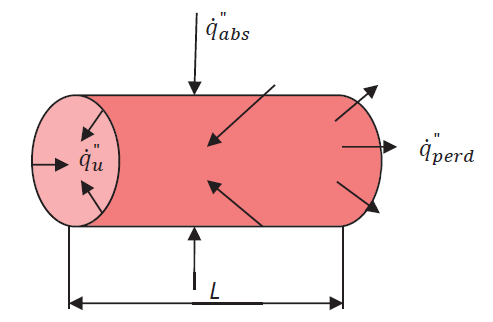
\includegraphics[scale=0.8]{images/receptor_para_modelo.png}}
	{\label{fig:receptormodelo}}
\end{figure}


La expresión para el cálculo de la radiación absorbida se muestra en la ec.\(\eqref{eq:qabs}\). 

\begin{equation}
    \dot{q}^{"}_{abs}= \eta_{opt}(\theta) \cdot Cg \cdot DNI \cdot \eta_{sombras} \cdot \eta_{bordes} \label{eq:qabs}
\end{equation}

El rendimiento óptico \(\eta_{opt}\), las pérdidas geométricas \(\eta_{bordes}\) y las pérdias por sombras, \(\eta_{sombras}\) son valores conocidos o que pueden calcularse para cada momento en función de la geometría del receptor y la disposicón de los concentradores en el campo solar. \(Cg\) es el factor de concentración y también es conocido a partir de la geometría del conjunto concentrador-receptor. Finalmente, \(DNI\) es la radiación normal incidente. La ec.\(\eqref{eq:qu}\) permite hallar al calor tranferido desde el tubo abosrbedor a temperatura \(T_{ro}\), al fluído térmico a temperatura \(T_{f}\):

\begin{equation}
    \dot{q}^{"}_{u}(x)= U_{rec} \cdot [T_{ro}(x)-T_{f}(x)] \label{eq:qu}
\end{equation}

donde \(U_{rec}\) es el ooeficiente global de transferencia de calor hacia el interior, cuya expresión se muestra en la ec.\(\eqref{eq:urec}\):

\begin{equation}
    U_{rec} = \frac{1}{\frac{1}{h_{int}} + \frac{D_{ro}\cdot(\frac{D_{ro}}{D_{ri})})}{2\cdot k_{rec}}} \label{eq:urec}
\end{equation}

Como aproximación se considera que \(U_{rec}\) es constate a lo largo de la longitud del tubo \((W/m^{2}\cdot K)\). \(D_{ro}\) y \(D_{ri}\) son el diámetro exterior e interior \((m)\) respectivamente del tubo absorbedor. \(h_{int}\) es el coeficiente de transferencia de calor convectivo hacia el interior \((W/m^{2}\cdot K)\) y \(k_{rec}\) es conductivdad del material del receptor, en \((W/m\cdot K)\)

Para las pérdidas se calculan mediante la ec.\(\eqref{eq:qperd}\) de calor se tendrá en cuenta un término radiativo, con temperaturas de 4o grado y otro convectivo de 1er grado. 

\begin{equation}
    \dot{q}^{"}_{perd}(x)= \sigma \cdot \varepsilon_{ext} \cdot (T_{ro}^{4}(x)-T_{ext}^{4}) + h_{hext} \cdot (T_{ro}(x)-T_{ext}) \label{eq:qperd}
\end{equation}

donde \(\sigma\) es la constante de Stefan-Boltzmann (5.67x10-8 W/m2K4), \(\varepsilon_{ext}\) es la emisividad del tratamiento superficial exterior y \(h_{hext}\) es el coeficiente de convección exterior. Estas dos últimas constantes son características de cada receptor y variables, por ejemplo, en función de las condiciones de degradación del recubrimiento selectivo o del viento exterior. Deben ser halladas experimentalmente en laboratorio.

La última ecuación necesaria es la ec.\(\eqref{eq:deltaT}\), donde se calcula el incremento de temperatura que experimenta el fluido considerando despreciables los cambios en energía cinética y un calor específico constante, \(c_{p}\) (J/Kg·K). Denominando \(T_{f}(x)\) a la tempertura del fluido en la sección a distancia \(x\) de la entrada y \(T_{fe}\) a la temperatura del fluido a la entrada, tenemos:

\begin{equation}
    \pi \cdot D_{ro} \cdot x \cdot \dot{q}^{"}_{abs} \cdot \eta(x)= \dot{m} \cdot c_{p} \cdot (T_{f}(x)-T_{fe}) \label{eq:deltaT}
\end{equation}\\

En esta última ecuación aparece el rendimiento integral hasta una sección a una distancia \(x\) de la entrada, \(\eta(x)\). Finalmente, a partir del rendimiento local, dado por la ec.\(\eqref{eq:rendimientolocal}\) podemos calcular el rendimiento integral mediante la ec.\(\eqref{eq:rendimientointegral}\).

\begin{equation}
    \eta_{x}(x) = \frac{\dot{q}^{"}_{u}(x)}{\dot{q}^{"}_{abs}} \label{eq:rendimientolocal}
\end{equation}

\begin{equation}
    \eta(x) = \frac{\int_{0}^{x}\eta_{x}(x)dx}{\int_{0}^{x}dx} \label{eq:rendimientointegral}
\end{equation}

donde desarrollando \(\eta_{x}(x)\) según la ec.\(\eqref{eq:etax}\):

\begin{equation}
    \eta_{x}(x) = \eta(x) + \eta'(x)\cdot x  \label{eq:etax}
\end{equation}

y normalizando la distancia a la unidad con la variable adimensional \(x^{*}=x/L\), obtenemos la ecuación integral ec.\(\eqref{eq:rendimientonormalizado}\):

\begin{equation}
    \eta(x^{*}) = 1 - \frac{\int_{0}^{x^{*}} \dot{q}^{"}_{perd}(dx^{*})\cdot dx^{*}}{\dot{q}^{"}_{abs}\cdot dx^{*}} \label{eq:rendimientonormalizado}
\end{equation}

La resolución de esta ecuación requiere un largo desarrollo en el que se introducen nuevos factores característicos del sistema y que puede encontrarse en la obra de referencia, por lo que la omitiremos aquí. Pese a la complejidad de la expresión final obtenida, que dificulta extraer conclusiones de manera directa, el modelo incorpora todos los parámetros característicos del sistema y lo hace manteniendo su sentido físico. A partir de la solución se puede obtener una expresión para el modelo local (rendimiento en una sección determinada del absorbedor) y una expresión para el modelo de colector completo, es decir, un rendimiento integral a lo largo de todo el absorbedor. Esta última es la que nos interesa. A continuación se presenta la ecuación del Modelo de 4º Orden completo del colector en la ec.\(\eqref{eq:modelocompleto}\) y sucesivamente las ecuaciones que definen sus parámetros:

\begin{equation}
    \eta(x^{*}) = \frac{\eta_{0} \cdot g'(Z)}{1-g'(Z)} \cdot \frac{1}{NTU \cdot x^{*}} \cdot \left(e^{\frac{1-g'(Z)}{g'(Z)}\cdot NTU \cdot x^{*}} - 1\right) - \frac{\eta_{0}^2}{6} \cdot \frac{g''(Z)}{g'(Z)} \cdot NTU^{2} \cdot x^{*^{2}} - \frac{\eta_{0}^{3}}{24} \cdot \frac{g'''(Z)}{g'(Z)} \cdot NTU^{3} \cdot x^{*^{3}}
    \label{eq:modelocompleto}
\end{equation}

\begin{equation}
    \eta_{0} = 1 - (f_{1} \cdot Z + f_{2} \cdot Z^{2} + f_{3} \cdot Z^{3} + f_{4} \cdot Z^{4})
    \label{eq:rendimiento0}
\end{equation}

\begin{equation}
    Z = \eta_{0} + \frac{1}{f_{0}} 
    \label{eq:zeta}
\end{equation}

\begin{equation}
    g(Z) = -\left(1+\frac{1}{f_{0}}\right)+(1+f_{1})\cdot Z + f_{2}\cdot Z^{2} +  f_{3}\cdot Z^{3} + f_{4}\cdot Z^{4} 
    \label{eq:gdezeta}
\end{equation}

\begin{equation}
    g'(Z) = 1 + f_{1} + 2 \cdot f_{2} \cdot Z + 3 \cdot f_{3} \cdot Z^{2} + 4 \cdot f_{4} \cdot Z^{3} 
    \label{eq:gprimadezeta}
\end{equation}

\begin{equation}
    g''(Z) = 2 \cdot f_{2} \cdot Z + 6 \cdot f_{3} \cdot Z + 12 \cdot f_{4} \cdot Z^{2} 
    \label{eq:g2primadezeta}
\end{equation}

\begin{equation}
    g'''(Z) = 6 \cdot f_{3} + 24 \cdot f_{4} \cdot Z
    \label{eq:g3primadezeta}
\end{equation}

\begin{equation}
    g^{IV}(Z) = 24 \cdot f_{4}
    \label{eq:g4primadezeta}
\end{equation}

\begin{equation}
    f_{1} = \frac{4 \cdot \sigma \cdot \varepsilon_{ext} \cdot T_{ext}^{3} + h_{ext}}{U_{rec}}
    \label{eq:f1}
\end{equation}

\begin{equation}
    f_{2} = 6 \cdot T_{ext}^{2} \cdot \left(\frac{\sigma \cdot \varepsilon_{ext}}{U_{rec}} \right) \cdot \left(\frac{\dot{q}^{"}_{abs}}{U_{rec}}\right) 
    \label{eq:f2}
\end{equation}

\begin{equation}
    f_{3} = 4 \cdot T_{ext} \cdot \left(\frac{\sigma \cdot \varepsilon_{ext}}{U_{rec}} \right) \cdot \left(\frac{\dot{q}^{"}_{abs}}{U_{rec}}\right)^{2} 
    \label{eq:f3}
\end{equation}

\begin{equation}
    f_{4} = \left(\frac{\sigma \cdot \varepsilon_{ext}}{U_{rec}} \right) \cdot \left(\frac{\dot{q}^{"}_{abs}}{U_{rec}}\right) 
    \label{eq:f4}
\end{equation}

Para la resolución de este modelo es preciso conocer previamente diferentes parámetros, muchos de los cuales pueden obtenerse directamente de las característias físicas y materiales con los que está construido el HCE. De especial importancia son \(\varepsilon_{ext}\) y \(h_{ext}\) pues son dos coeficientes que de forma global vienen a caracterizar las pérdidas energéticas del receptor. Para obtener las ecuaciones que los caracterizan se parte de la expresión del coeficiente global del pérdidas al exterior dada por la ec.\(\eqref{eq:uext}\) de la siguiente forma:

\begin{equation}
    U_{ext} = h_{hext} + \sigma \cdot \varepsilon_{ext} \cdot \left(T_{ro}^2 + T_{ext}^2 \right) \cdot \left(T_{ro} + T_{ext} \right)
    \label{eq:uext}
\end{equation}

Es necesario realizar ensayos de laboratorio bajo diferentes condiciones de viento (\(W_{spd}\)) y temperatura exterior (\(T_{ext}\)) para obtener el flujo de calor de pérdidas y calcular así dos expresiones del tipo \(\varepsilon_{ext}(T_{ext},W_{spd})\) y \(h_{ext}(T_{ext},W_{spd})\). Para este trabajo se emplean los valores obtenidos en \cite{barberofresnoDesarrolloModeloTeorico2018} a partir de \cite{burkholderHeatLossTestingSolel2008}, \cite{burkholderHeatLossTesting2009} y \cite{kutscherGenerationParabolicTrough2012}.

A partir de este modelo de 4º Orden se realiza un desarrollo que permite obtener dos modelos simplificados de colector completo: el Modelo de Primer Orden y el Modelo Simplificado.

\section{Modelo de Primer Orden}

La ec.\(\eqref{eq:primerorden}\) presenta el Modelo de Primer Orden. Para llegar a ella resuelve la ec.\(\eqref{eq:rendimiento0}\) despreciando monomios a partir de segundo grado, con lo que se puede sustituir el rendimiento a la entrada del absorbedor, \(\eta_{0}\), por su valor aproximado dado en la ec.\(\eqref{eq:rendimiento0aproximado}\):

\begin{equation}
    \eta(x^{*}) = \left[1-\frac{\dot q''_{crit}}{\dot q''_{abs}}\right] \cdot \frac{1}{NTU_{perd} \cdot x^{*}} \cdot \left(1-e^{-NTU_{perd}\cdot F'_{crit}\cdot x^{*}}\right) 
    \label{eq:primerorden}
\end{equation}

\begin{equation}
    \eta_{0} = F'_{crit} \cdot \left[1-\frac{\dot q''_{crit}}{\dot q''_{abs}}\right] 
    \label{eq:rendimiento0aproximado}
\end{equation}

En esta ecuación se han reagrupado variables en diferentes términos que cuentan con sentido físico. De este modo, se definen:

\begin{equation}
    \dot q''_{crit} = \sigma \cdot \varepsilon_{ext} \cdot \left(T^{4}_{fe}- T^{4}_{ext}\right)+h_{hext} \cdot \left(T^{4}_{fe}- T^{4}_{ext}\right)
    \label{eq:qcrit}
\end{equation}

\begin{equation}
    U_{crit} = 4 \cdot \sigma \cdot \varepsilon_{ext} \cdot T^{3}_{fe} + h_{hext}
    \label{eq:ucrit}
\end{equation}

\(\dot q''_{crit}\) y \(U_{crit}\) son valores de referencia en el estudio del comportamiento del colector pues cuando \(\dot q''_{abs}\) y \(U_{rec}\) se aproximan a ellos el rendimiento del colector se hace nulo. Por otra parte, \(F'_{crit}\) se asemeja al parámetro empleado en el modello desarrolado por Hottel y Whillier en \cite{1022085/DVRL97SH}.

\begin{equation}
    F'_{crit} = \frac{1}{\frac{4 \cdot \sigma \cdot \varepsilon_{ext} \cdot T^{3}_{fe}}{U_{rec}} + \frac{h_{ext}}{U_{rec}} +1} = \frac{1}{\frac{U_{crit}}{U_{rec}}+1}
    \label{eq:fcrit}
\end{equation}

El Modelo de Primer Orden presenta la ventaja de que el cálculo de \(\eta(x^{*})\) es explícito. Más adelante veremos cómo repercute esto en la reducción del coste computacional. Por otro lado, también nos ofrece una forma de calcular un valor aproximado del rendimiento a la entrada del colector, \(\eta_{0}\).

\section{Modelo simplificado}
Si se desarrolla por Taylor la funcion exponencial del Modelo de Primer Orden, se trunca por el segundo término y se sustituye \(\dot q''_{abs}\) por su expresión en función de \(DNI\) se obtiene la ec.\(\eqref{eq:modelosimplificado}\) para el cálculo del rendimiento total en el receptor mediante el Modelo Simplificado:

\begin{equation}
    \eta_{T} = F'_{crit} \cdot \left[1 - \frac{\dot q''_{crit}}{\dot q''_{abs}}\right] = \frac{F'_{crit}}{Cg} \cdot \left[Cg \cdot IAM \cdot cos(\theta) \cdot \eta_{opt,pico} \cdot \eta_{sombras} \cdot \eta_{bordes} - \frac{h_{ext}\cdot (\bar{T}_{f}-\bar{T}_{ext})}{DNI} - \frac{\sigma \cdot \varepsilon_{ext}\cdot(\bar{T}^{4}_{f}-\bar{T}^{4}_{ext})}{DNI}\right] 
    \label{eq:modelosimplificado}
\end{equation}

Esta ecuación es más parecida a la encontrada en otros modelos de diferentes autores, como por ejemplo en \cite{hottelEvaluationFlatplateSolar1955} o \cite{fraidenraichImprovedSolutionsTemperature1997a}, pero con dependencia de \(T^{4}\) lo cual tiene mayor sentido físico al esperarse que las pérdidas radiativas sean dominantes en situaciones de media y alta concentración.

\section{Aplicabilidad de los modelos}
Aunque en el caso del Modelo de 4º Orden no se ha realizado ninguna simplificación para la resolución de la ecuación caracterítica, sí que se han hecho las siguientes consdiraciones que limitan su aplicacion: 
* Se ha considerdo que los parametros característicos \(U_{rec}\), \(\varepsilon_{ext}\), \(h_{ext}\) y \(Cp\) son constantes a lo largo de toda la longitud del receptor. Se considerará que esto es aceptable para longitudes inferiores a 100 m tal y como se indica en el desarrollo del modelo. 
* Se supone uniformidad del flujo de radiación sobre el tubo absorbedor. Para tecnología CCP se acepta esta hipótesis. 
* La caracterización de los tubos absorbedores empleados en CCP es compatible con el desarrollo del modelo basada en un tubo desnudo (para los que posteriormente se emplearán unos coeficientes de trasmisión de calor adecuados para los tubos con cubierta de vidrio). 
* La suposición de fluido incompresible en la que se desprecia el término de pérdida de carga y de energía cinética sobre el término energético es adecuada para plantas que operan con aceite térmico dado que los circuitos están presurizados para mantener en todo momento el fluido en estado líquido y los caudales de operación tienen un número de Reynolds medio. 
* El flujo puede suponerse uniforme en el interior del tubo absorbedor. 
* Dada la longitud real del tubo absorbedor en una planta CCP, puede despreciarse el efecto de transmisión de calor longitudinal. 

Según lo visto, el modelo resulta aplicable a la simulación de un campo solar de concentradores cilindroparabólicos bajo las condiciones normales de operación. Por otro lado, la simulación se realizará también para el cálculo con intervalos horarios en los que se supondrá condiciones estacionarias de planta y se descartarán aquellos periodos de arranque y parada o cambios abruptos en los que las inercias propias del sistema y la intervención de los operadores de planta producirían que el comportamiento instantáneo no se correspondiese con el simulado.

El Modelo de Primer Orden presenta mayores restricciones, especialmente en los rangos de operación aceptables (no deben ser próximos a los valores críticos definidos en la ec.\(\eqref{eq:ucrit}\) y \(\eqref{eq:qcrit}\)), siendo sus resultados algo menos precisos en general.

El Modelo Simplificado solo es válido además para longitudes de receptor más reducidas.
